% asset_id: FA22LinearCombinationsOfIndependentVariablesTikZ-004
% unit_code: FA22
% topic_code: FA22-LINCOMB
% topic_id: FA22LinearCombinationsOfIndependentVariables
% source: Phase 1 visual placeholder register
% purpose: Right-tail inverse normal
\documentclass[tikz,border=10pt]{standalone}
\usepackage{amsmath}
\usepackage{tikz}
\begin{document}
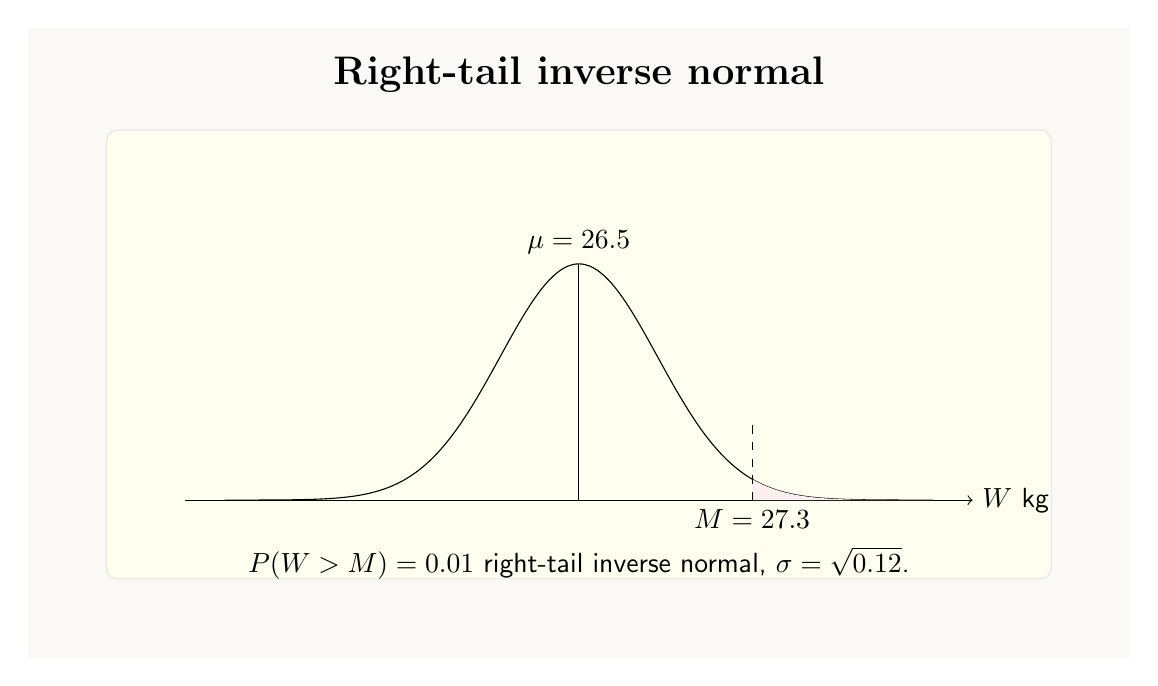
\begin{tikzpicture}[font=\sffamily]
\fill[fill={rgb,255:red,250;green,249;blue,246}] (-1,-1) rectangle (13,7);
\node[font=\bfseries\Large] at (6,6.4) {Right-tail inverse normal};
\draw[rounded corners, fill={rgb,255:red,255;green,255;blue,240}, draw={rgb,255:red,229;green,229;blue,234}] (0,0) rectangle (12,5.7);

\draw[->] (1,1)--(11,1); \node[right] at (11,1) {$W$ kg};
\draw[smooth, domain=1.5:10.5, samples=100] plot (\x,{1+3*exp(-0.5*(\x-6)^2)});
\fill[fill={{rgb,255:red,251;green,239;blue,239}}] plot[domain=8.2:10.5,samples=80] (\x,{1+3*exp(-0.5*(\x-6)^2)}) -- (10.5,1) -- (8.2,1) -- cycle;
\draw (6,1)--(6,4); \node[above] at (6,4) {$\mu=26.5$};
\draw[dashed] (8.2,1)--(8.2,2.0); \node[below] at (8.2,1) {$M=27.3$};
\node at (6,0.2) {$P(W>M)=0.01$ right-tail inverse normal, $\sigma=\sqrt{0.12}$.};

\end{tikzpicture}
\end{document}
